\section{Trajectory generation}
\label{sec:trajectory_generation}


This section outlines the various approaches we employ
for real time trajectory generation
(\cref{sub:base_motion}, \cref{sub:arm_motion}).
Furthermore, we explain how the symbolic actions introduced
in \cref{fig:software_overview}, 
looking for products
(\cref{sub:look_for_product}), pick
(\cref{sub:picking}) and place (\cref{sub:place})
are realized and we
explain how they use the trajectory generation approaches.

\subsection{Navigation of the base}
\label{sub:base_motion}
To navigate the mobile base in the store, we employ the ROS MoveBase framework, configured with A* as the global and Timed-Elastic-Bands as the local planner~\cite{rosmann2017integrated}.
We record an environment map including static obstacles prior to deployment.
Additionally, we manually define keep-out
areas to prevent the robot from going into unsafe or crowded areas, such as checkout zones. The local planner uses the environment map and online lidar sensor information for avoiding collisions with static and moving obstacles, such as humans.

\subsection{Motion of the arm}
\label{sub:arm_motion}
To generate the arm motions (and base during picking),
we employ \ac{fabrics}. Fabrics is based on
behavior composition, defined as differential
equations in manifolds, which enables safe
real-time planning at high frequencies
\cite{ratliff2023fabrics,van2022geometric,Spahn2023}. Since
\ac{fabrics} is a local, reactive trajectory generation
method, we require global guidance to perform complex
symbolic actions, such as product picking or placing. The global
guidance for fabrics consists of a sequence of
local goals, where we only continue to the next goal if the
previous goal has been reached. In \cref{sub:teaching} we
show how this sequence of goals, i.e., reference trajectory,
can be obtained by human teaching. In the following, we briefly explain how \ac{fabrics} works and how to use it.



\subsubsection{Method}
Requirements such as collision avoidance, joint-limit avoidance or self-collision avoidance are referred to in fabrics as behavioral components. Each component is represented as a differential equation of the form
$\M(\x,\xdot)\xddot+\f(\x,\xdot)=\nullvec$ on an appropriate
manifold \X{} of the configuration space \Q{}, where \M{} and \f{} are the importance metric and the forcing term respectively, and $\x$, $\xdot$ and $\xddot$ are the state, e.g., full configuration of the robot or end effector pose, and its derivatives in the manifold \X{}.
By respecting
simple construction rules, each behavioral component can be ensured to
be an optimization fabric, i.e., a dynamic system that is
stable by construction. All components can then be combined
in the robot's configuration space by applying the
operations of \textit{pullback} and \textit{summation}. In
the configuration space, we obtain one optimization fabrics
of the form $\M\qddot + \f = \nullvec$, where $\qddot$ is the second derivative of the configuration and $\M$ and $\f$ the resulting importance metric and forcing term, respectively.
We define goal states of the robotic arm as a set of
constraints $\Sc = \{\Con_1,\Con_i,\Con_n\}$ where each
constraint \Con{} is defined by the tuple
$\Con=(\fkarg{p},\fkarg{c},\x)$. Here, $\fkarg{p}$ is the forward
kinematics to the parent link, $\fkarg{c}$ the forward
kinematics to the child link, and $\x$ is the desired position
vector. These constraints are implemented in \ac{fabrics} as a forcing term with the
differential map $\map_{\textrm{goal}} = (\fkarg{c} - \fkarg{p}) -
\x$. On the manifold defined by this differential map, we
define the forcing potential $\forc$ that can be pulled at
forcing our optimization fabric as
$\M\qddot+\f+\der{\q}{\forc} = 0$.
The final policy is then defined as the solution to the
damped differential equation as
\begin{equation}
  \qddot = -\M^{-1}(\f + + \mat{B}\qdot + \der{\q}{\forc}),
  \label{eq:fabrics_policy}
\end{equation}
where $\mat{B}$ is a positive definite damping matrix.
For further details, we refer readers to \cite{Spahn2023}.

The key advantages of \ac{fabrics} are their fast computation and flexibility to
compose behaviours and define the desired goal in a manifold, rather than being
fixed to defining a target configuration or end-effector pose. For
example, some tasks may require aligning the end-effector
to face a specific point, while
the actual position along the line is of little importance, see
\cref{fig:look_for_product}.
Similarly, some products, like a can, can be grasped from many directions and one may only need to specify a subset of desired grasping poses, e.g., the grasp height and that the grasp should be perpendicular to the vertical axis, but not the specific approach direction.


\begin{figure}[b]
  \centering
  \begin{subfigure}[b]{0.5\linewidth}
    \centering
    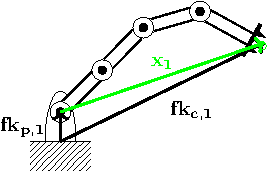
\includegraphics[width=1\textwidth]{one_constraint.pdf}
    \caption{}
    \label{subfig:one_goal_constraint}
  \end{subfigure}%
  \begin{subfigure}[b]{0.5\linewidth}
    \centering
    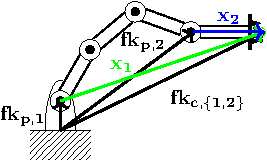
\includegraphics[width=1\textwidth]{two_constraints.pdf}
    \caption{}
    \label{subfig:two_goal_constraints}
  \end{subfigure}
  \caption{Goal constraints for \ac{fabrics}. In (a), 
  the only constraint is defined by $\Con_1 = (\fkarg{p,1},
  \fkarg{c,1}, \x_1)$.
  In (b), a second constraint is added as
   $\Con_2 = (\fkarg{p,2}, \fkarg{c,2}, \x_2)$ to align the
   end-effector horizontally.}
  \label{fig:goal_constraints}
\end{figure}

\subsubsection{Safety}
\label{ssub:safety}

An important aspect of applications of robotics solutions to
human-shared environments is \textit{safety} and
failure-free operation during an extended amount of time.
For the latter, the most important aspect is that
joint-limits and self-collision is avoided at all times,
because these can lead to hardware shutdowns.
In \ac{fabrics}, these constraints are achieved by defining a joint-limit
avoidance and self-collision avoidance components as
described above, making these failures virtually impossible.
Safety, however, is more complex to achieve, as it requires an
accurate environment model and a reliable prediction of
humans and their individual joints. In this work, we instead
opted for safety through compliance during arm motion, i.e.,
the robot is compliant to external forces. This is achieved
by tracking the desired acceleration output from
\cref{eq:fabrics_policy} with a low-level controller that
outputs the torques for the individual joints.
Specifically, we use a
PI controller that tracks the velocity that is obtained by
integrating the desired acceleration. This approach allows
ensuring that collisions are non-harming to the robot and its
environments. 

\subsubsection{Usage} As an example, a reaching problem, where the
end-effector should be at a certain position is defined by
$\Con_{\textrm{ee}} = (\fkarg{0},\fkarg{ee},\x_\textrm{ee})$,
where $\fkarg{0}$ is the forward kinematics to the base link of
the robot and $\x_\textrm{ee}$ the desired position of the
end-effector in the base link frame.\cref{fig:goal_constraints} shows two examples of composing goal states by constraints.

A problem we encountered when picking products with only the arm, is that the arm's workspaceis limited w.r.t. the shelf's size. This in combination with variability in base position or product location, often resulted in the product being out of reach or requiring difficult arm configurations close to joint limits.
%As the workspace of the arm is quite limited, base navigation can be quite inaccurate, and product locations might be disturbed by other customers,
Therefore, during picking, we augment arm motion by integrating the forward motion of the base as a pseudo-prismatic joint to the kinematic chain. This can be easily done in \ac{fabrics} by appending the base motion to the state vectors \q{}, \qdot{}, and \qddot{}, see \cref{fig:base_motion}. 


\subsection{Look for a product}
\label{sub:look_for_product}
Looking for the product is triggered as soon as the robot
base is in front of the shelf that is expected to
have the desired product. The camera frame is then located
at a position $\x_{\camera}$. The camera
must be pointed towards the expected product location, defined as
$\x_{\product}$. We can model this goal as two
constraints. First, the camera link should not move from its
current location, thus $\Con_1 =
(\fkarg{0},\fkarg{camera},\x_{\textrm{camera}})$. Secondly, the
camera should face the product location. We  compute the
ray connecting the camera and product location
$\x_{\textrm{ray}} = \x_{\product} - \x_{\camera}$ to 
define $\Con_2 = (\fkarg{flange}, \fkarg{end-effector},  \x_{\textrm{ray}})$
that aligns the end-effector with the
defined ray $\x_{\textrm{ray}}$, see
\cref{fig:look_for_product}.

\begin{figure}
  \begin{center}
    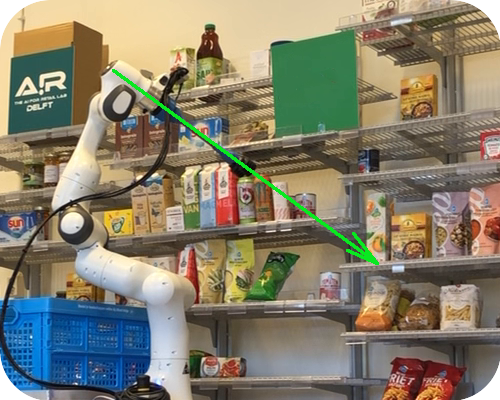
\includegraphics[width=0.55\linewidth]{look_for_item_wo.png}
  \end{center}
  \caption{Illustration of the orientation constraints for trajectory
  generation for look-for-product.}
  \label{fig:look_for_product}
\end{figure}


\subsection{Picking of a product}
\label{sub:picking}
To define a goal for picking products we use a combination of three constraints.
First, the position of the vacuum cup is determined by the
position of the product, thus $\Con_1 =
(\fkarg{0},\fkarg{suction-cup}, \x_{\textrm{suction}}, \weight_{\textrm{suction}})$. Secondly, we
limit  ourselves to picking products from the shelf, thus
constraining the end-effector to be perpendicular to the
shelf by defining $\Con_2 = (\fkarg{flange},\fkarg{end-effector},
\x_{\textrm{flange,end-effector}})$. Lastly, our gripper is composed of two
suction cups, which, depending on the product should align with a specific angle for executing the most reliable grasp. The desired alignment defines
our third constraint for the picking as $\Con_3 =
(\fkarg{suction1}, \fkarg{suction2}, \x_{\textrm{alignment}})$. Although it is possible to
program picking, including approach and retreat, as a sequence of this set of
constraints, it is difficult to capture all the nuances of
picking in the code. Therefore, we make use of a human operator to teach the robot the best trajectory to reliably pick specific products, following the 
learning-from-demonstration paradigm
\cite{celemin2022interactive}. Teaching has proven an effective way to generate sequences of the previously mentioned
constraints thus encoding the human understanding of the picking problem into recorded trajectories. We explain the process of
recording and playing back trajectories in detail in \cref{sub:teaching}. 
%

%

\subsection{Placing of a product}
\label{sub:place}

Placing the product consists of four phases. The robot navigates
to a configuration to its right or to its left depending on
whether it was a right-sided pick or a left-sided pick.
Then, it moves above the crate facing downwards. This is
defined by two constraints, $\Con_1 =
(\fkarg{0},\fkarg{end-effector},
\x_{0,end-effector}, 1)$ and $\Con_2 =
(\fkarg{flange},\fkarg{end-effector},
\x_{flange,end-effector})$.
The product is placed by moving the arm downwards until an
external force, from touching the crate's bottom
or an already placed product, is detected. This triggers the gripper
release and goal change to the homing
position ready for the next product.
% In
% case, the robot is commanded with a goal defined in the
% configuration space, we limit motion to the arm. All other
% goals are composed as a union of \textit{goal-constraints}.
% A goal-constraint is a defined by a desired distance vector
% between two links on the kinematic chain. 








